\documentclass{article}
\usepackage{graphicx, fancyhdr, amsmath}
\usepackage[margin=0.6in, top=1in]{geometry}
\usepackage{float}
\usepackage[absolute, overlay]{textpos}
\usepackage[colorlinks=true, linkcolor=blue]{hyperref}

\pagestyle{fancy}
\fancyhf{}
\renewcommand{\headrulewidth}{0pt}

\fancyhead[L]{
\begin{textblock*}{2cm}(0.3in,0.1in)  % {block width} (x-coordinate, y-coordinate)
    
\includegraphics[width=2cm]{NEW LOGO.png}  % Example image placeholder
\end{textblock*}
}
\fancyhead[R]{Math Success Program, UCLA}
\fancyfoot[R]{Created for the MSP by Asmi Kawatkar}

\fancypagestyle{plain}{
}


\title{Review Sheet: Related Rates}
\date{}
\author{}

\begin{document}
\maketitle
\vspace{-0.75in}
\section*{Content Review}
\subsection*{Overview}
Related rates problems involve finding the rate at which one quantity is changing using information about other known quantities. 

Most related rates problems you will encounter at the level of Math 31A/B will require roughly the following steps in their solutions:
\begin{enumerate}
    \item \textbf{Relationship:} Establish a relationship between the variables. \\Relationships/Equations to consider: Trigonometric, Equations of area, surface area and volume of common geometrical shapes, mathematical similarity, equation of speed etc.
    \item \textbf{Derivative}: Take a derivative of that relationship (often with respect to time). This step involves implicit differentiation. Review this concept if you need to before attempting these problems. 
    \item \textbf{Substitution:} Substitute known values (sometimes this step will also involve using the relationship established before to find some value that you need)
\end{enumerate}

\subsection*{Helpful Equations}

\textit{Geometry}

$$\text{Area of a circle} = \pi r^2$$

$$ \text{Volume of sphere} = \frac{4}{3}\pi r^2$$

$$\text{Surface area of sphere} = 4 \pi r^2$$

$$\text{Volume of cone or pyramid} = \frac{1}{3}\times \text{base area} \times \text{height}$$

$$\text{Area of curved surface of cone} = \pi r \times \text{slant height}$$

$$\text{Arc length of circle} = r\theta \text{ \hspace{3pt}($\theta$ in radians)}$$

$$\text{Area of sector of circle} = \frac{r^2\theta}{2} \text{ \hspace{3pt}($\theta$ in radians)}$$

\noindent\textit{Trigonometry}
$$\tan \theta = \frac{\sin \theta}{\cos \theta}$$
$$\cos^2\theta + \sin^2\theta = 1$$
$$1 + \tan^2\theta = \sec^2\theta$$
$$\cot^2\theta + 1 = \csc^2\theta$$

\noindent Skip to \hyperref[WorkedProblems]{Worked Problems}.

\subsection*{Resources}

\textit{Mathematical Similarity}
\begin{itemize}
    \item \href{https://www.khanacademy.org/math/geometry-home/similarity}{Khan Academy: Similarity (Geometric)}
    \item \href{https://www.youtube.com/watch?v=BI-rtfZVXy0}{Video: Similarity (Khan Academy, 10 min)}
    \item \href{https://mathbitsnotebook.com/Geometry/Similarity/SMSimilarPractice.html}{Practice Problems: Similarity of Triangles (Basic)}
    \item \href{https://cdn.kutasoftware.com/Worksheets/PreAlg/Similar%20Figures.pdf}{Practice Problems: Similarity of Shapes (Advanced)}
\end{itemize}


\noindent\textit{Implicit Differentiation}
\begin{itemize}
    \item MSP Review Sheet on Implicit Differentiation
    \item \href{https://www.khanacademy.org/math/ap-calculus-ab/ab-differentiation-2-new/ab-3-2/a/implicit-differentiation-review#:~:text=In%20implicit%20differentiation%2C%20we%20differentiate,2%20%3D%201%20%E2%80%8D%20for%20example.}{Khan Academy: Implicit Differentiation}
    \item \href{https://tutorial.math.lamar.edu/classes/calci/implicitdiff.aspx}{Paul's Online Notes (With worked problems)}
\end{itemize}

\noindent\textit{Related Rates}
\begin{itemize}
    \item \href{https://youtu.be/I9mVUo-bhM8}{Video: Introduction to Related Rates (Organic Chemistry Tutor, 10 min) - with worked examples} 
    \item \href{https://youtu.be/ps-r4nti5Go}{Video: Related Rates - Conical Tank, Ladder \& Shadow, Calculus (Organic Chemistry Tutor) - with extensive worked examples}
    \item \href{https://www.math.ucdavis.edu/~kouba/CalcOneDIRECTORY/relatedratesdirectory/RelatedRates.html}{Practice Problems: UC Davis Math}
\end{itemize}


\subsection*{Acknowlegement}
Questions in the Worked Problems section of this sheet have been taken from external sources like \href{https://www.khanacademy.org/math/ap-calculus-ab/ab-diff-contextual-applications-new/ab-4-5/e/related-rates}{Khan Academy} and \href{https://tutorial.math.lamar.edu/classes/calci/relatedrates.aspx}{Paul's Online Notes}. All solutions have been created independently.

\pagebreak
\section*{Worked Problems}
\label{WorkedProblems}
\begin{enumerate}
    \item The radius $r(t)$ of a circle is increasing at the rate of 3 cm per second. At a certain instant $t_0$, the radius is 8 cm. What is the rate of change of the area $A(t)$ of the circle at that instant?
    \begin{figure}[H]
        \centering
        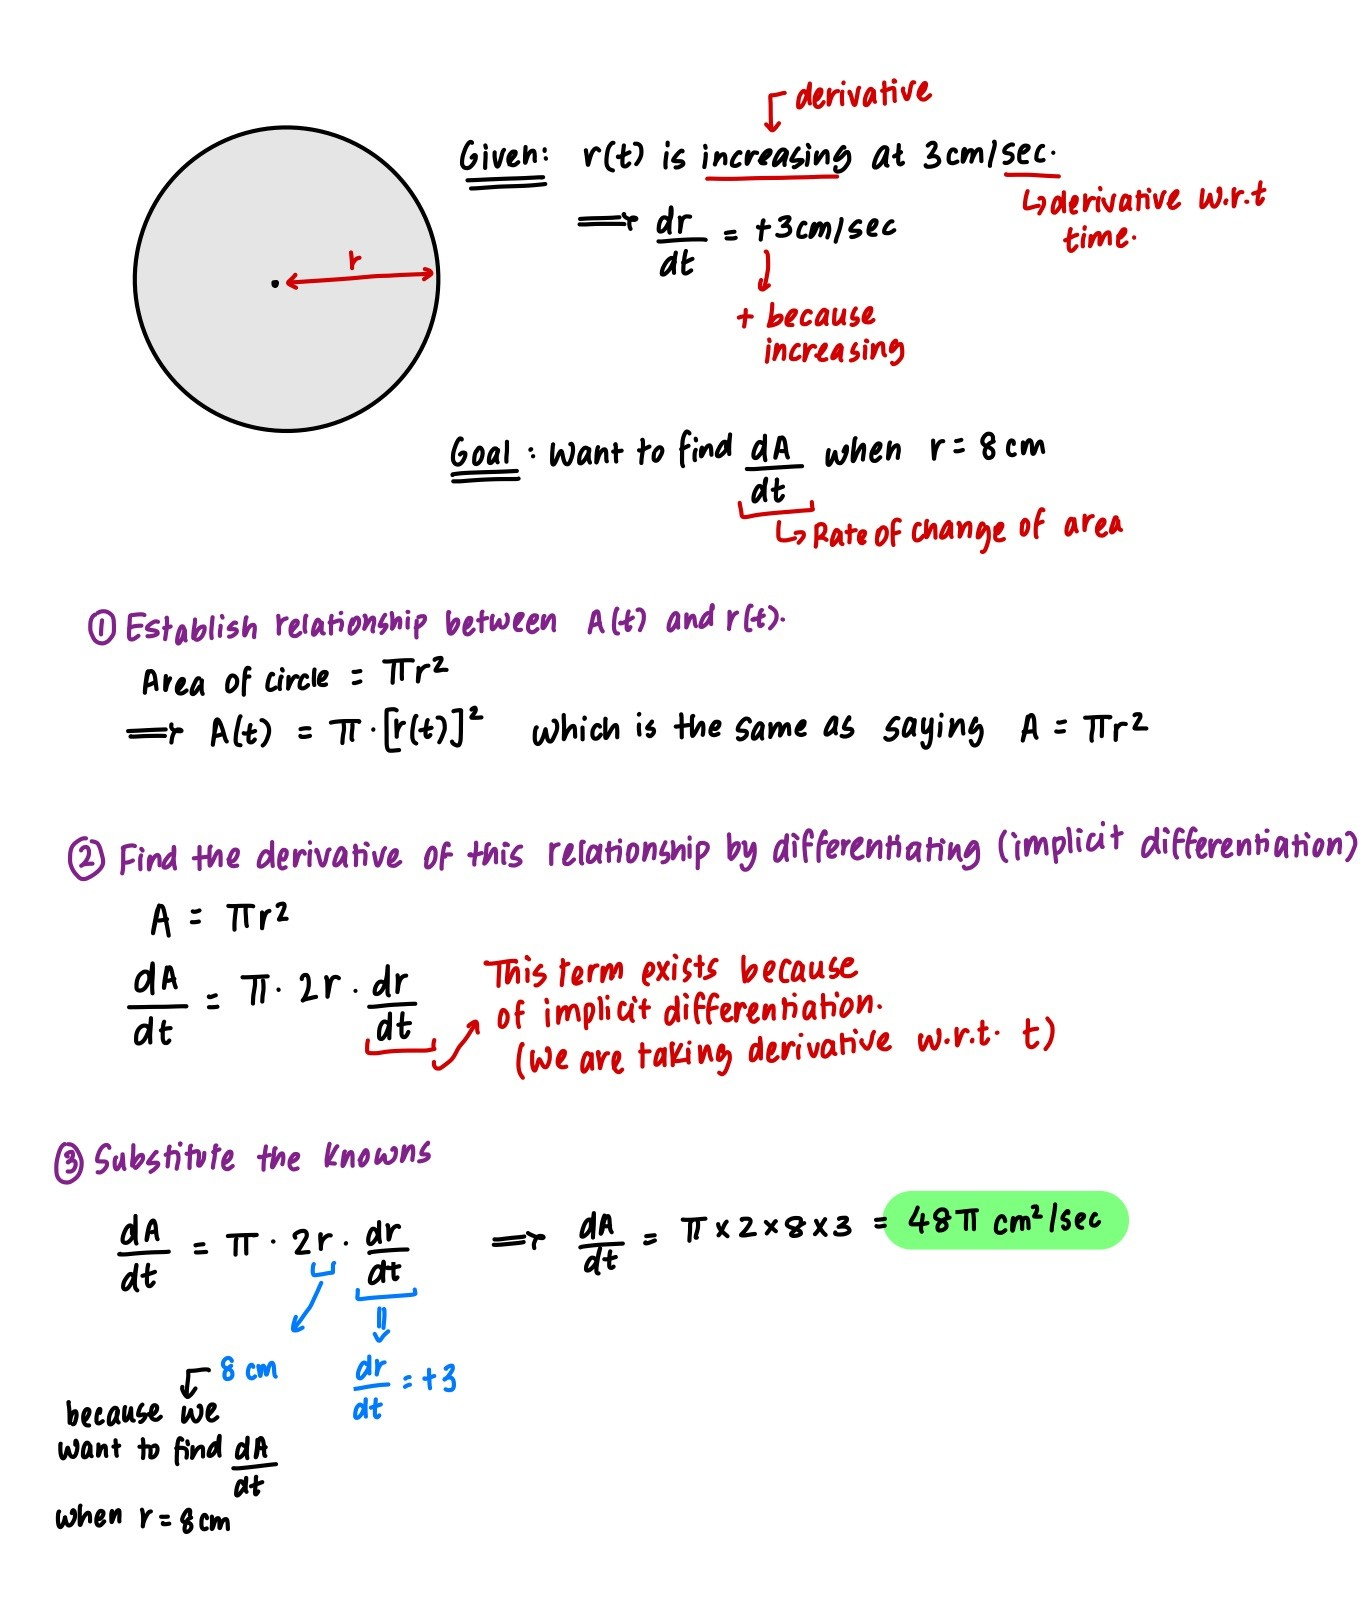
\includegraphics[width=0.8\linewidth]{Q1.jpg}
        \label{fig:Q1}
    \end{figure}
    
    \pagebreak
    \item A plane is 750 meters in the air flying parallel to the ground at a speed of 100 m/s and is initially 2.5 kilometers away from a radar station. At what rate is the distance between the plane and the radar station changing 
    \begin{enumerate}
        \item initially
        \item 30 seconds after it passes over the radar station 
    \end{enumerate}
     \begin{figure}[H]
        \centering
        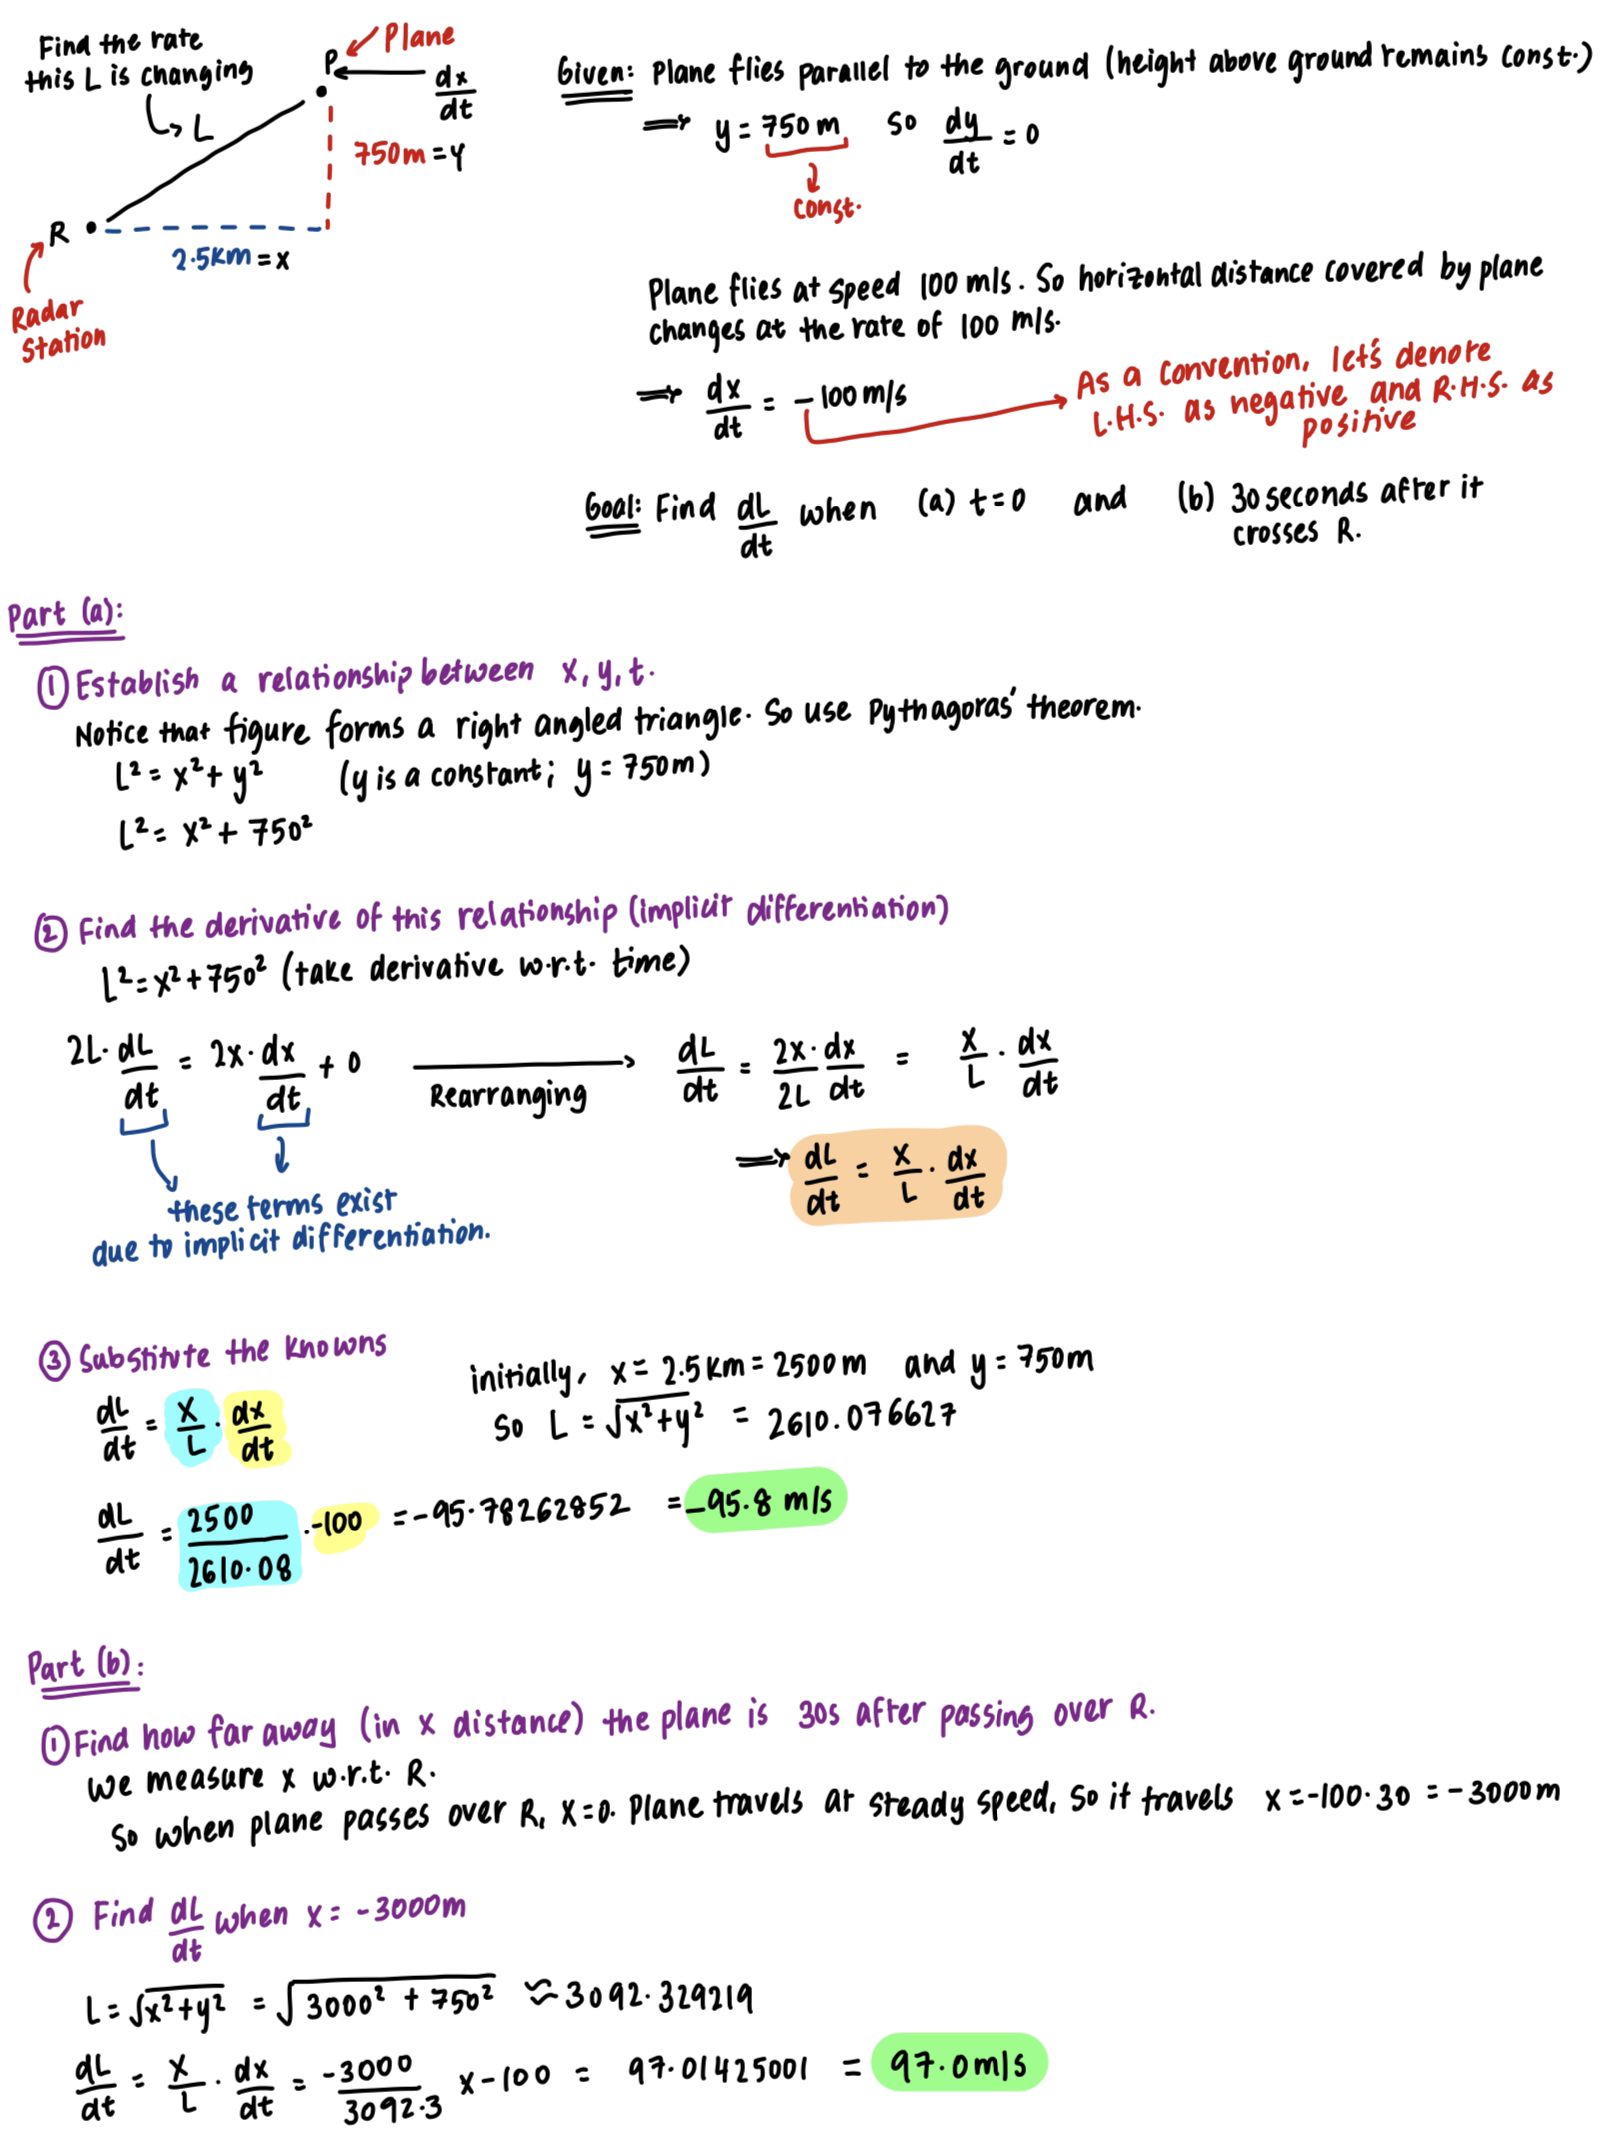
\includegraphics[width=0.85\linewidth]{Q2.jpg}
        \label{fig:Q2}
    \end{figure}
    \pagebreak
    \item Two people are at an elevator. At the same time one person starts to walk away from the elevator at a rate of 2 ft/sec and the other person starts going up in the elevator at a rate of 7 ft/sec. What rate is the distance between the two people changing 15 seconds later?
     \begin{figure}[H]
        \centering
        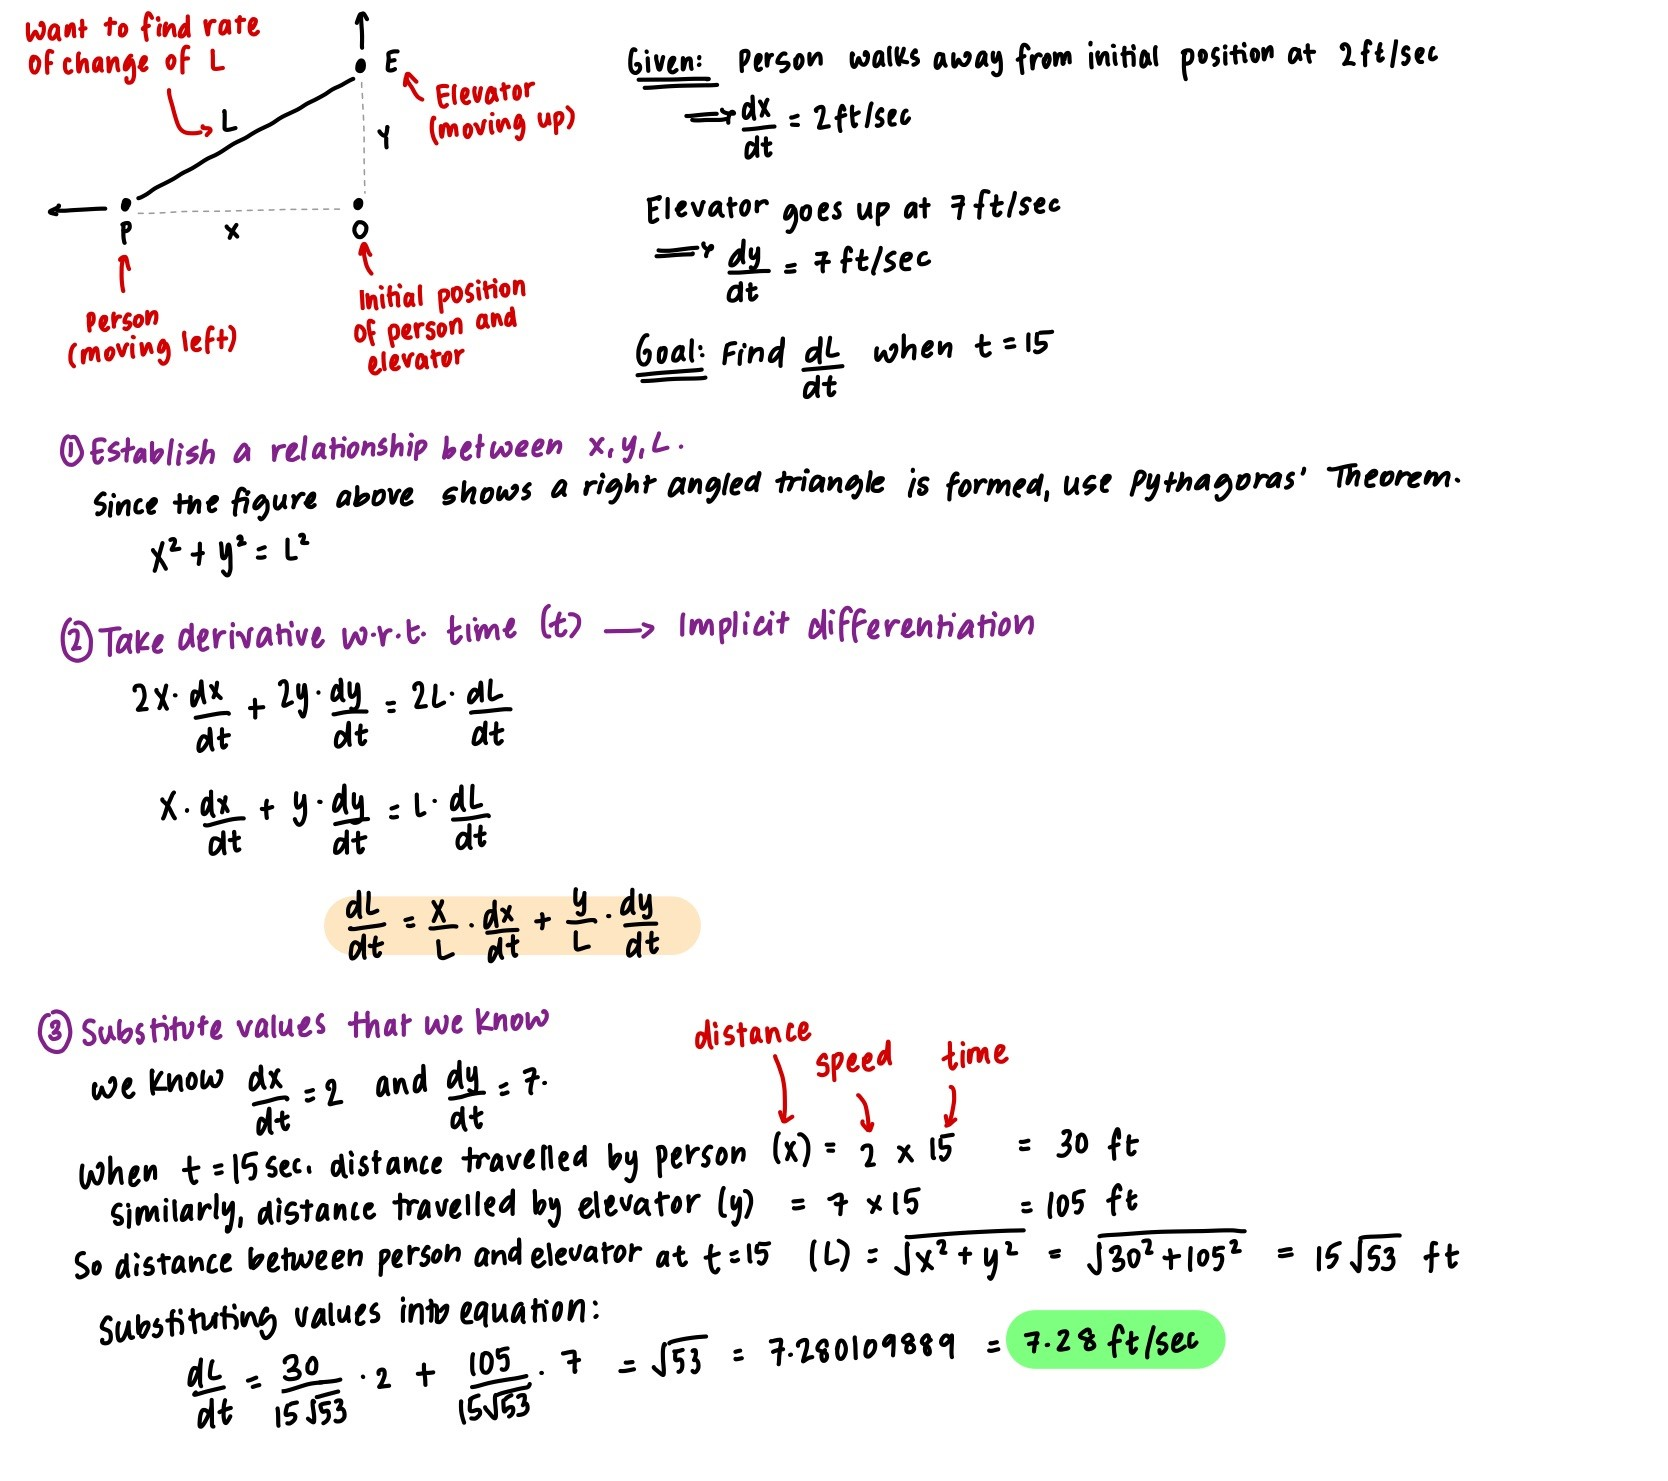
\includegraphics[width=\linewidth]{Q3.jpg}
        \label{fig:Q3}
    \end{figure}

    \pagebreak
    \item A tank of water in the shape of a cone is being filled with water at a rate of 12 m3/sec. The base radius of the tank is 26 meters and the height of the tank is 8 meters. At what rate is the depth of the water in the tank changing when the radius of the top of the water is 10 meters?
    \begin{figure}[H]
        \centering
        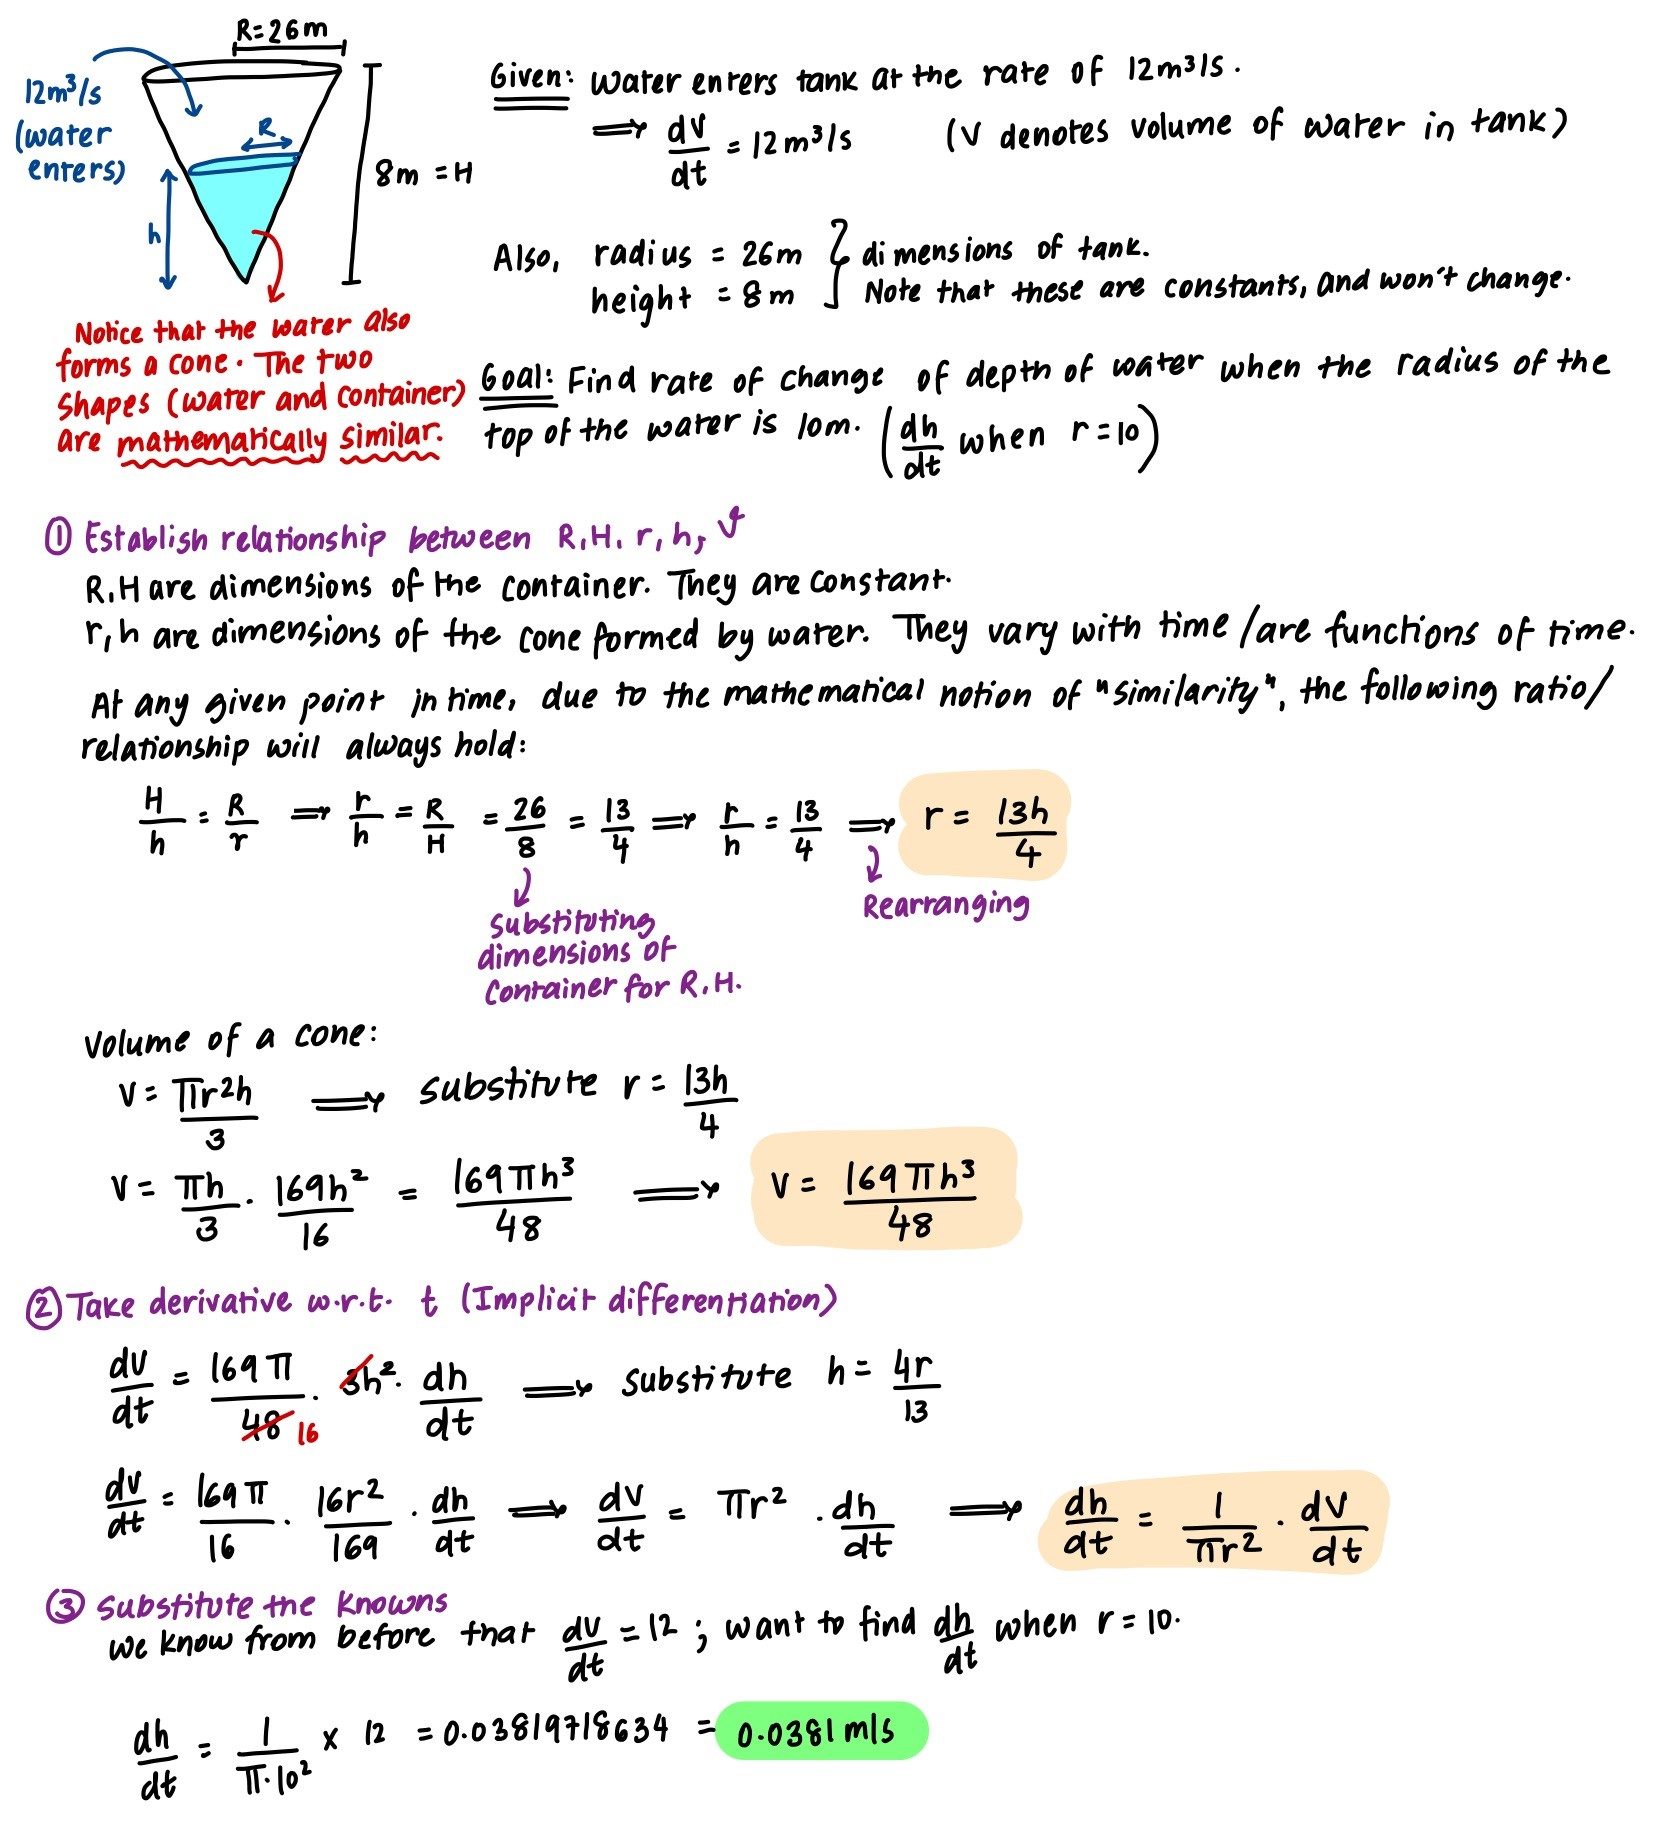
\includegraphics[width=\linewidth]{Q4.jpg}
        \label{fig:Q4}
    \end{figure}

    \pagebreak
    \item The angle of elevation is the angle formed by a horizontal line and a line joining the observer’s eye to an object above the horizontal line. A person is 500 feet way from the launch point of a hot air balloon. The hot air balloon is starting to come back down at a rate of 15 ft/sec. At what rate is the angle of elevation, $\theta$ changing when the hot air balloon is 200 feet above the ground? 

    \begin{figure}[H]
        \centering
        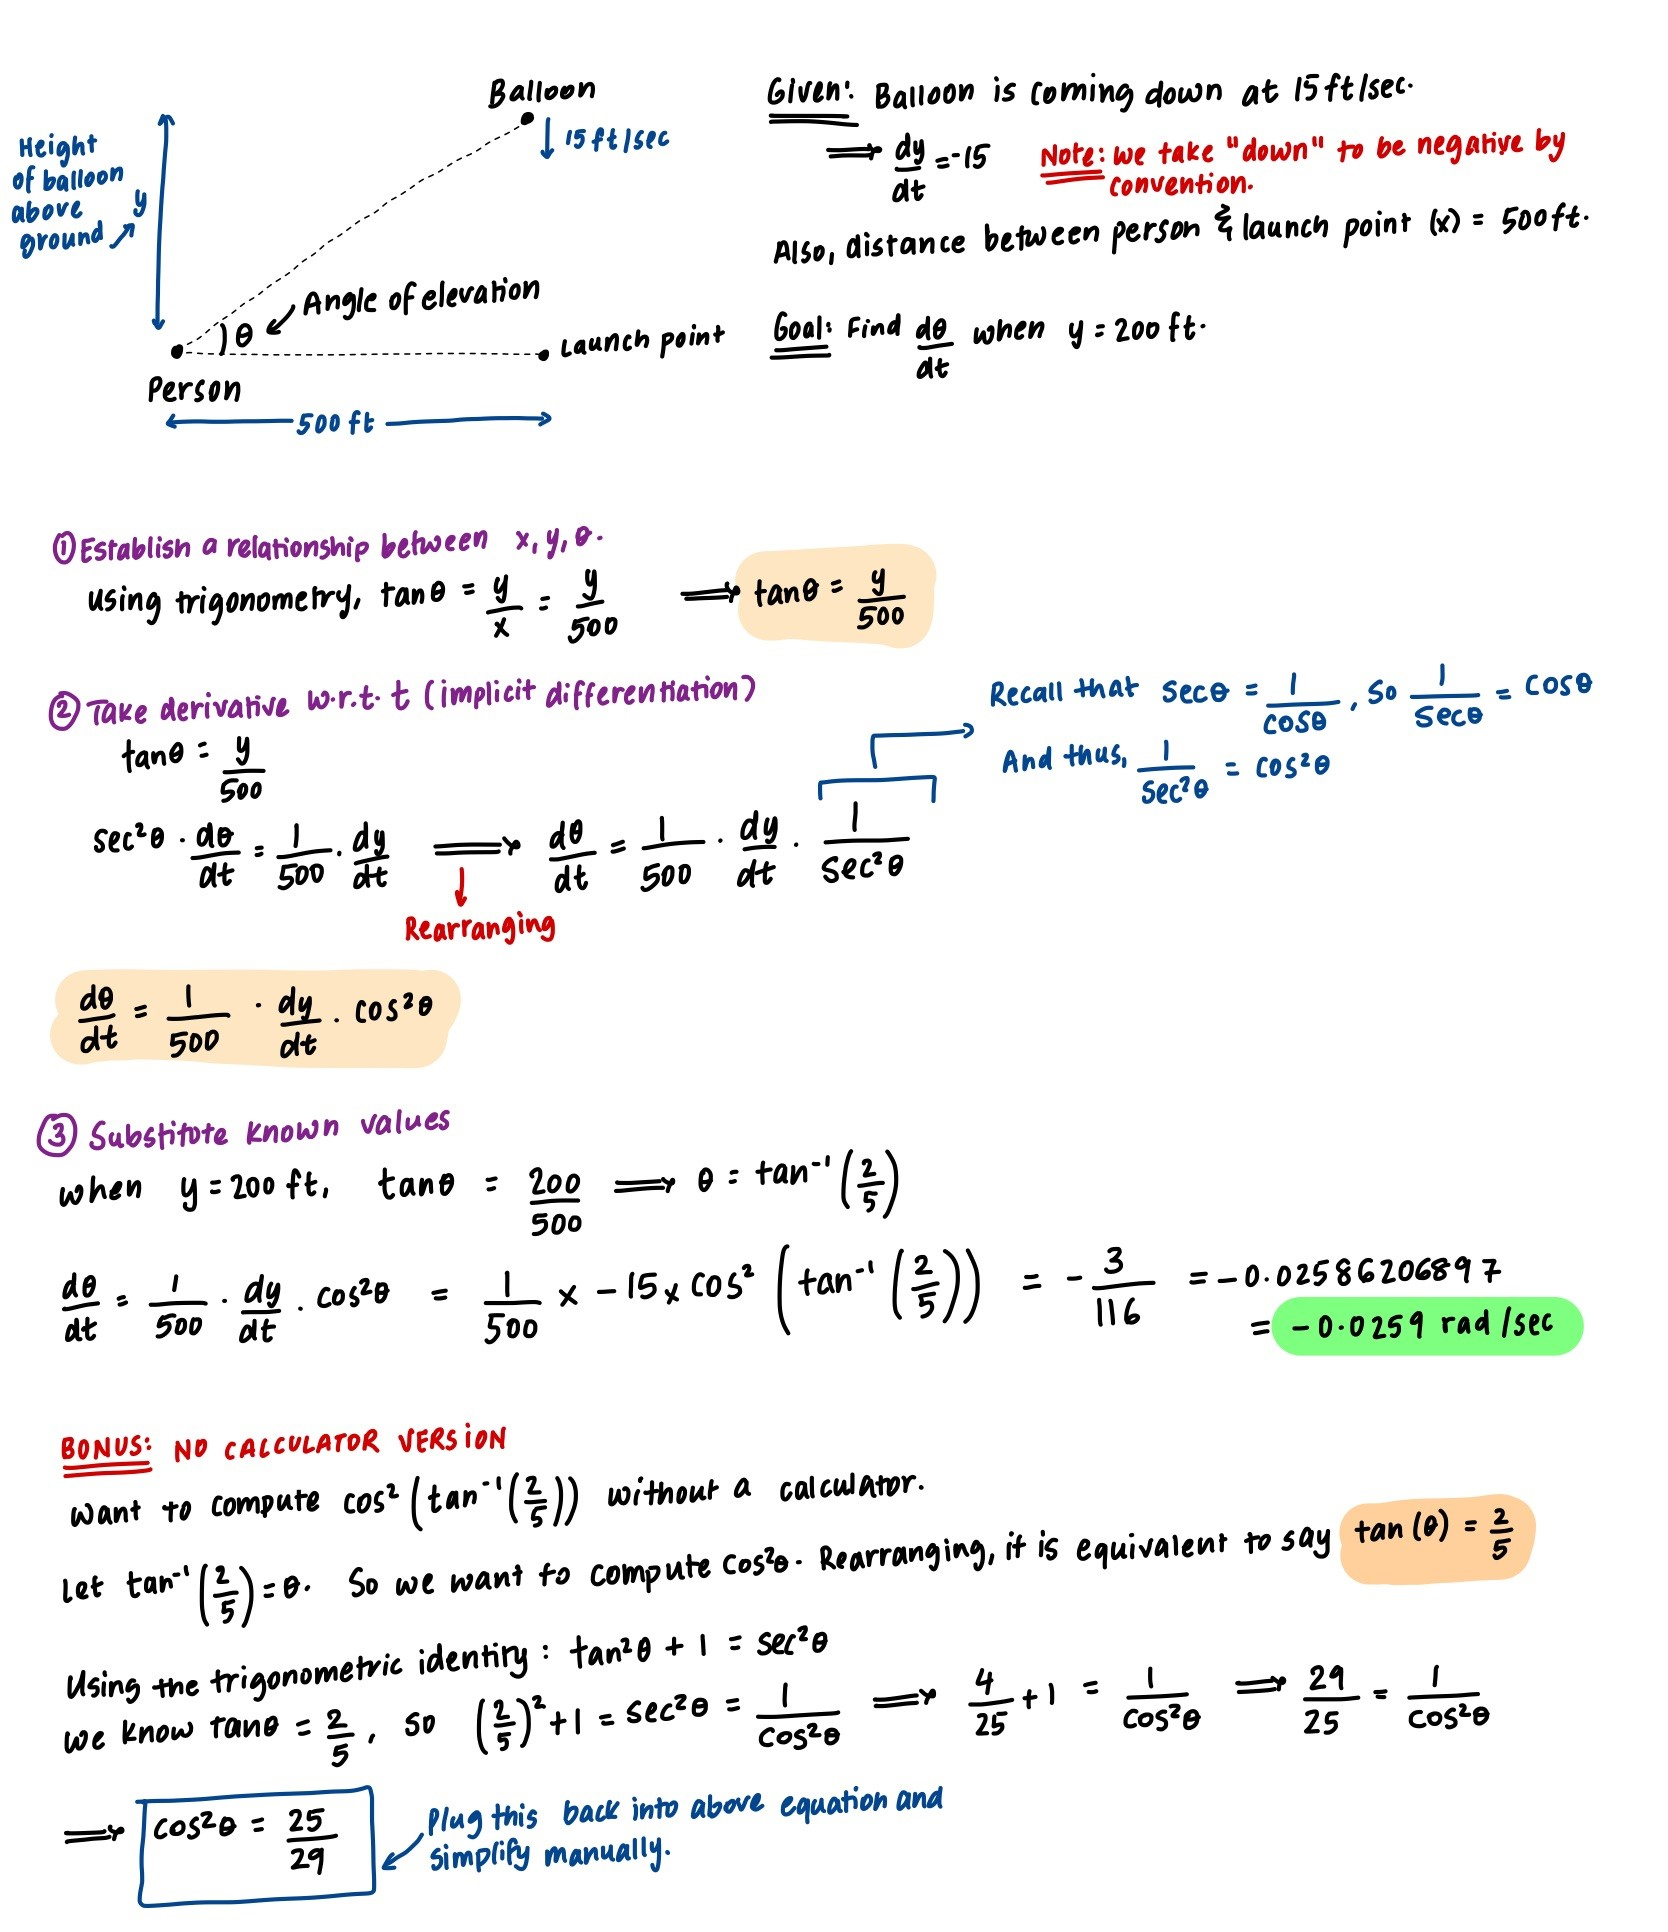
\includegraphics[width=0.98\linewidth]{Q5.jpg}
        \label{fig:Q5}
    \end{figure}
\end{enumerate}

\end{document}
